\subsection{Election November 6, 1900: *McKinley vs Bryan}
\begin{frame}[t]{Election November 6, 1900: *William McKinley}
\small
% McKinley
\begin{columns}[T, onlytextwidth]
\column{0.48\textwidth}
\vspace{-1em}
{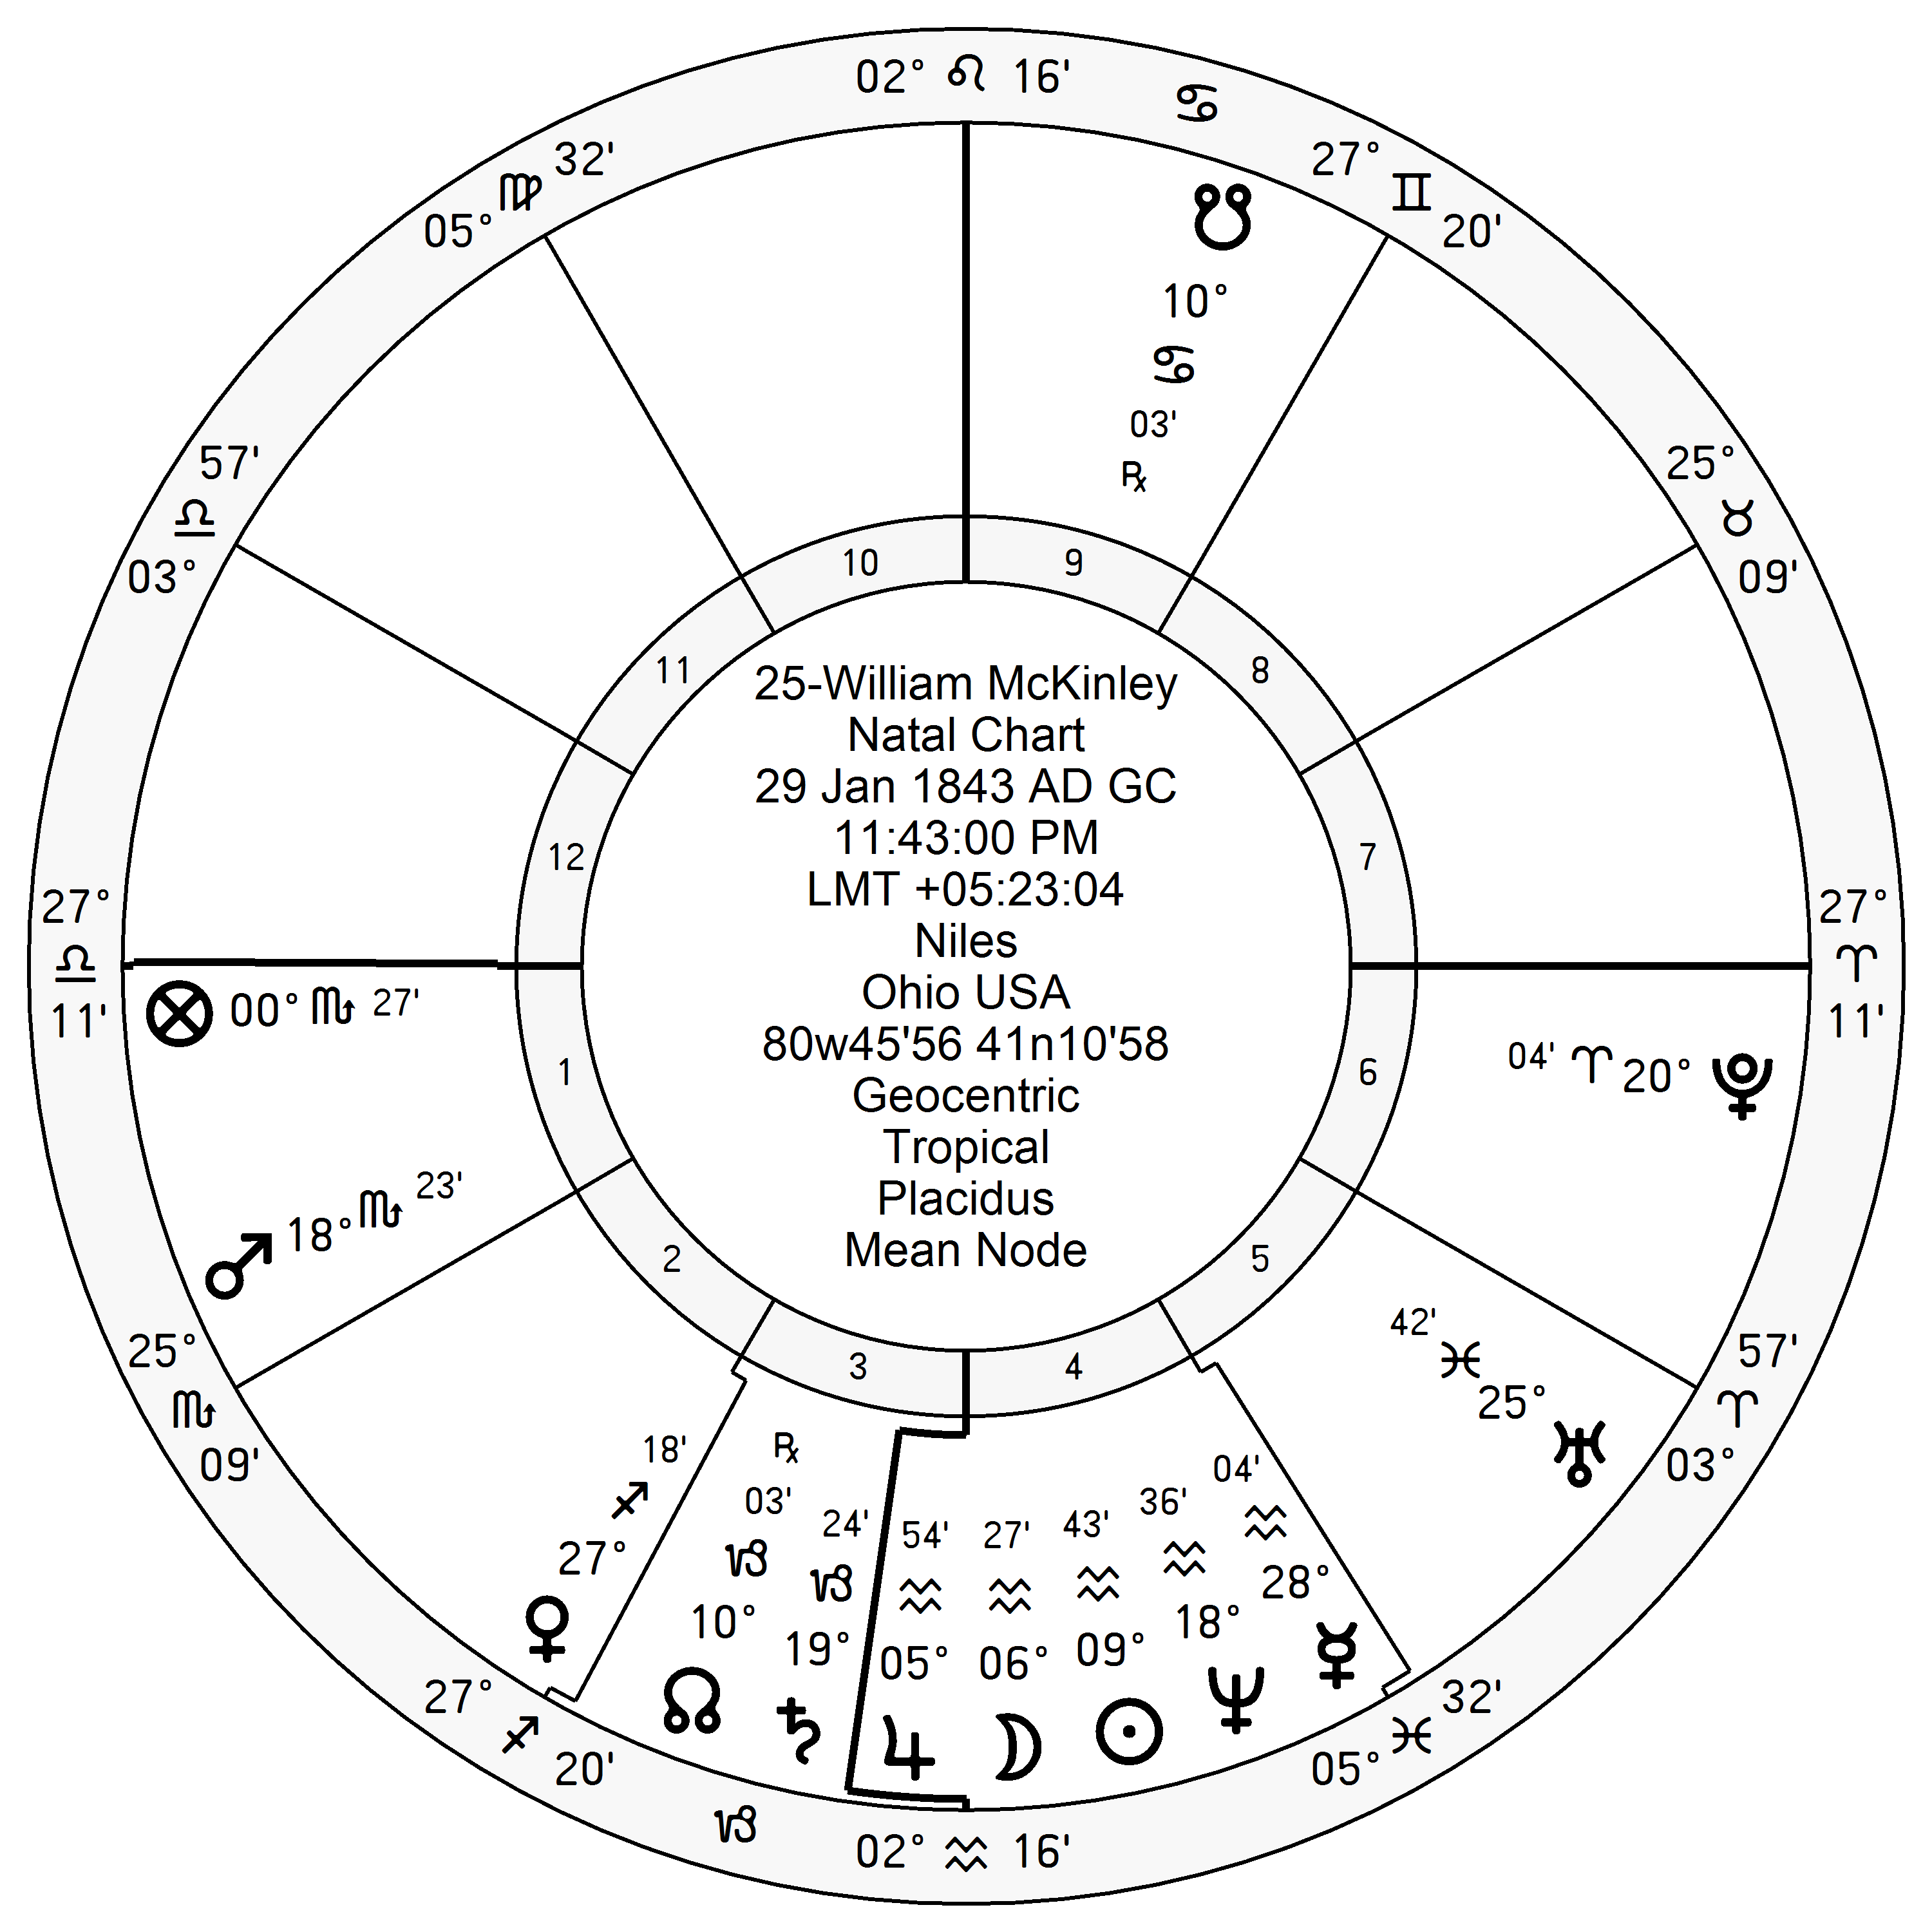
\includegraphics[width=0.9\textwidth]{charts/McKinley.png}}
\fontsize{7pt}{8pt}\selectfont

\Moon\, \Opposition\, P1, N10. The \Moon's combustion does not appear to create a problem; possibly protected by the \Jupiter\, \Conjunction. \\
\Mars\, \Opposition\, P10, \Square\, N10; \Square\, P1, in N1.

\column{0.48\textwidth}
\vspace{-1em}
{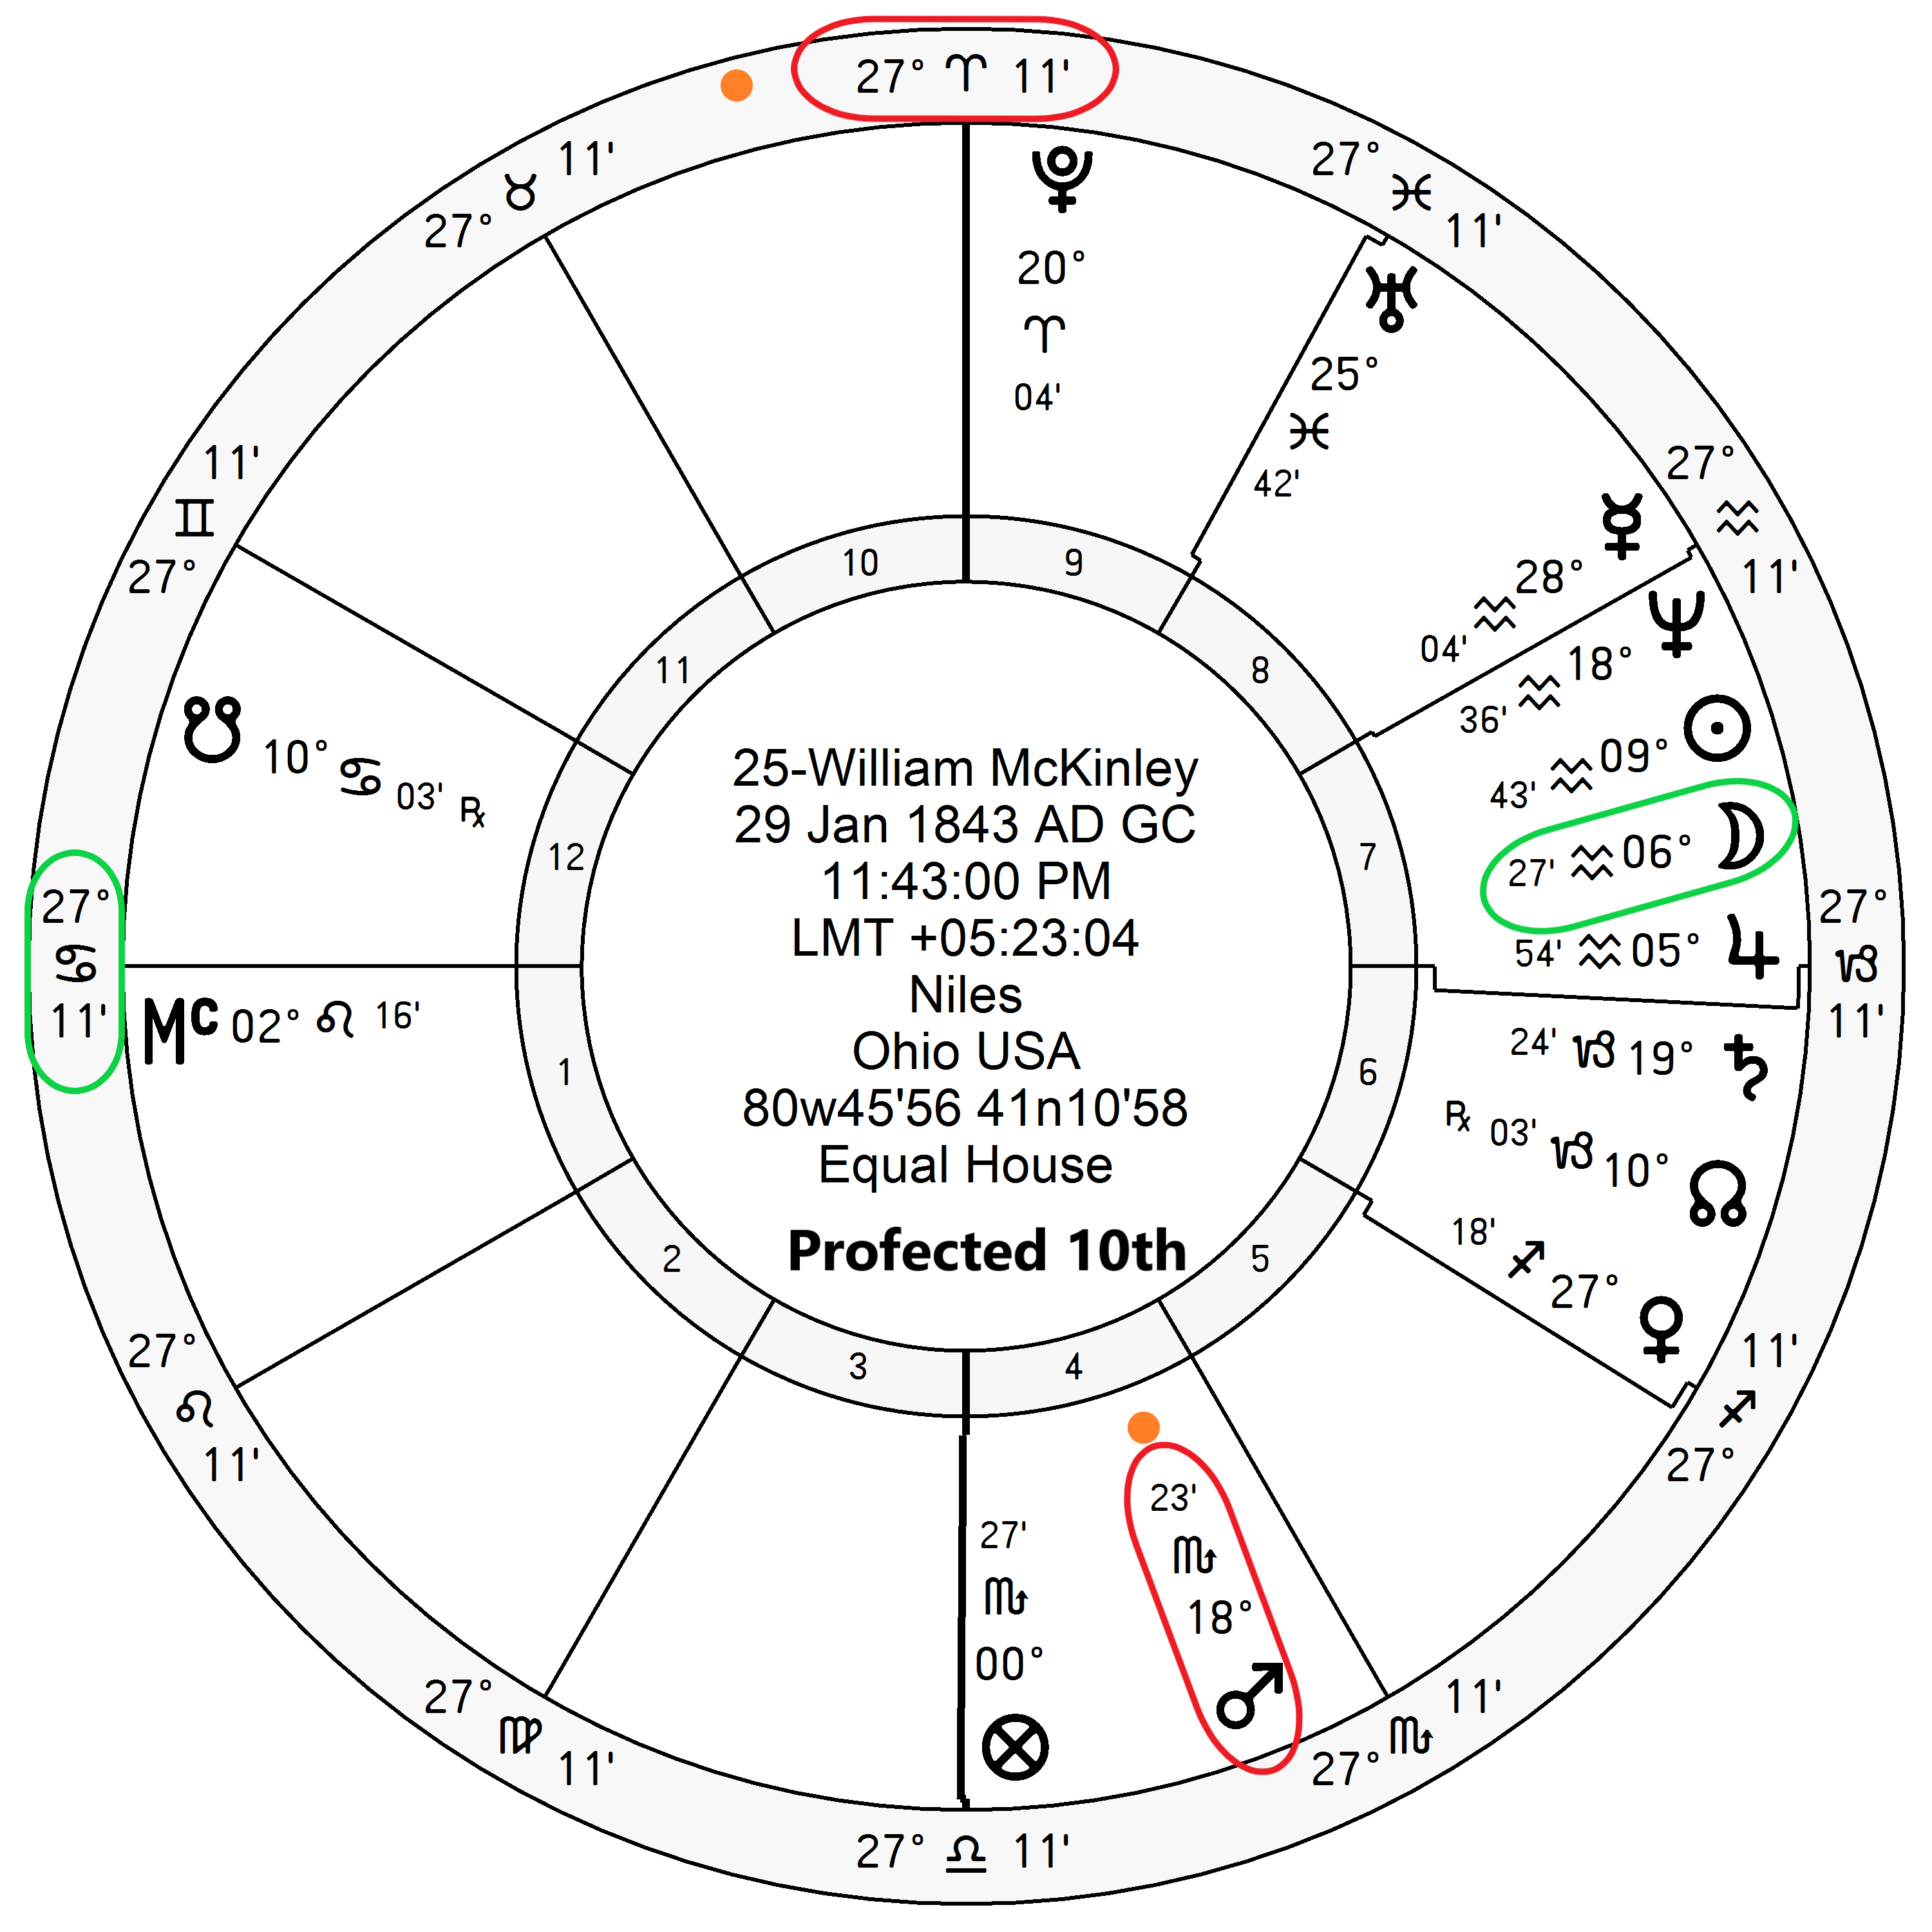
\includegraphics[width=0.9\textwidth]{charts/McKinley-Prof-10th.png}}
\textbf{\dgreen P1}=N9 
	$\Rightarrow$ \Moon\, $\Rightarrow$ \textbf{\red P7}/\textbf{\dgreen N4} \\
\textbf{\red P10=N7} 
	$\Rightarrow$  \Mars\, $\Rightarrow$  \textbf{\dgreen P4/N1} \\
PE=\textbf{\red P10/N7} 
	$\Rightarrow$  \Mars\, $\Rightarrow$  \textbf{\dgreen{P4/N1}}
\end{columns}
\end{frame}

% Bryan
\begin{frame}[t]{Election November 6, 1900: William Jennings Bryan}
\small
\begin{columns}[T, onlytextwidth]
\column{0.48\textwidth}
\vspace{-1em}
{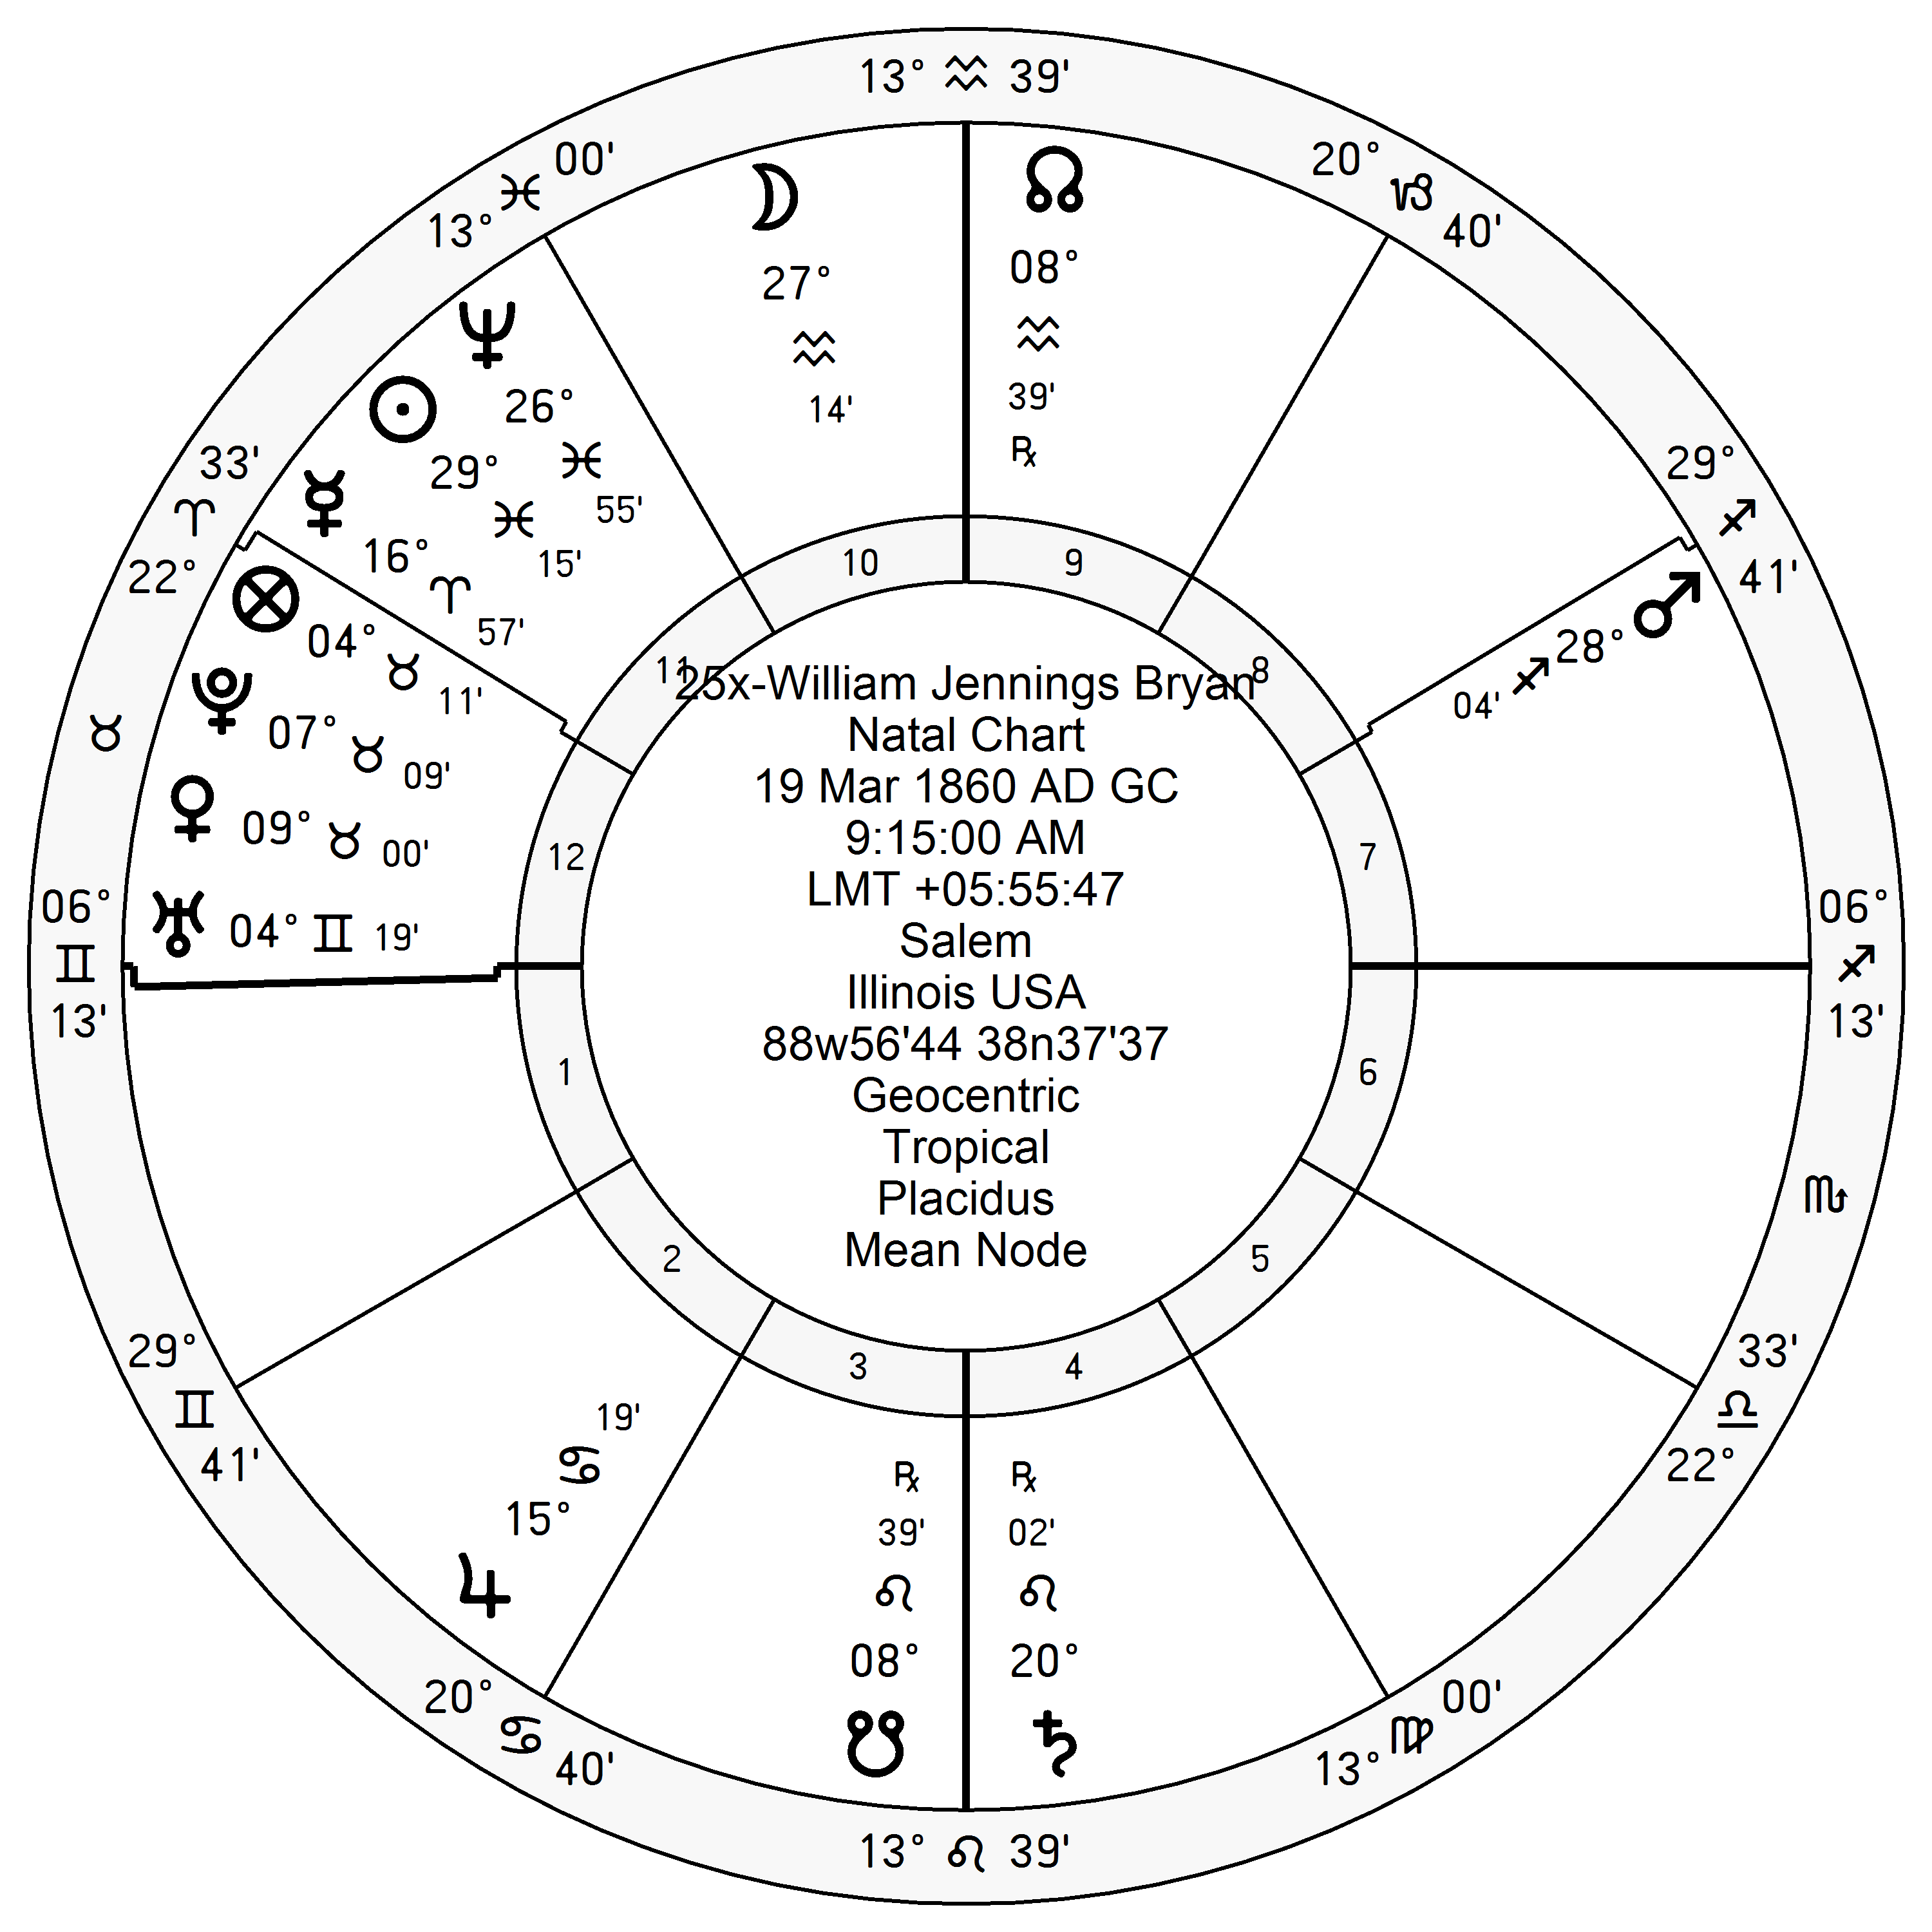
\includegraphics[width=0.9\textwidth]{charts/Bryan.png}}
\fontsize{8pt}{9pt}\selectfont

\Venus\, \Sextile\, P10, N10 \\
\Moon\, in N10, \Trine\, N1 \\
\Saturn\, \Opposition\, N10.

\column{0.48\textwidth}
\vspace{-1em}
{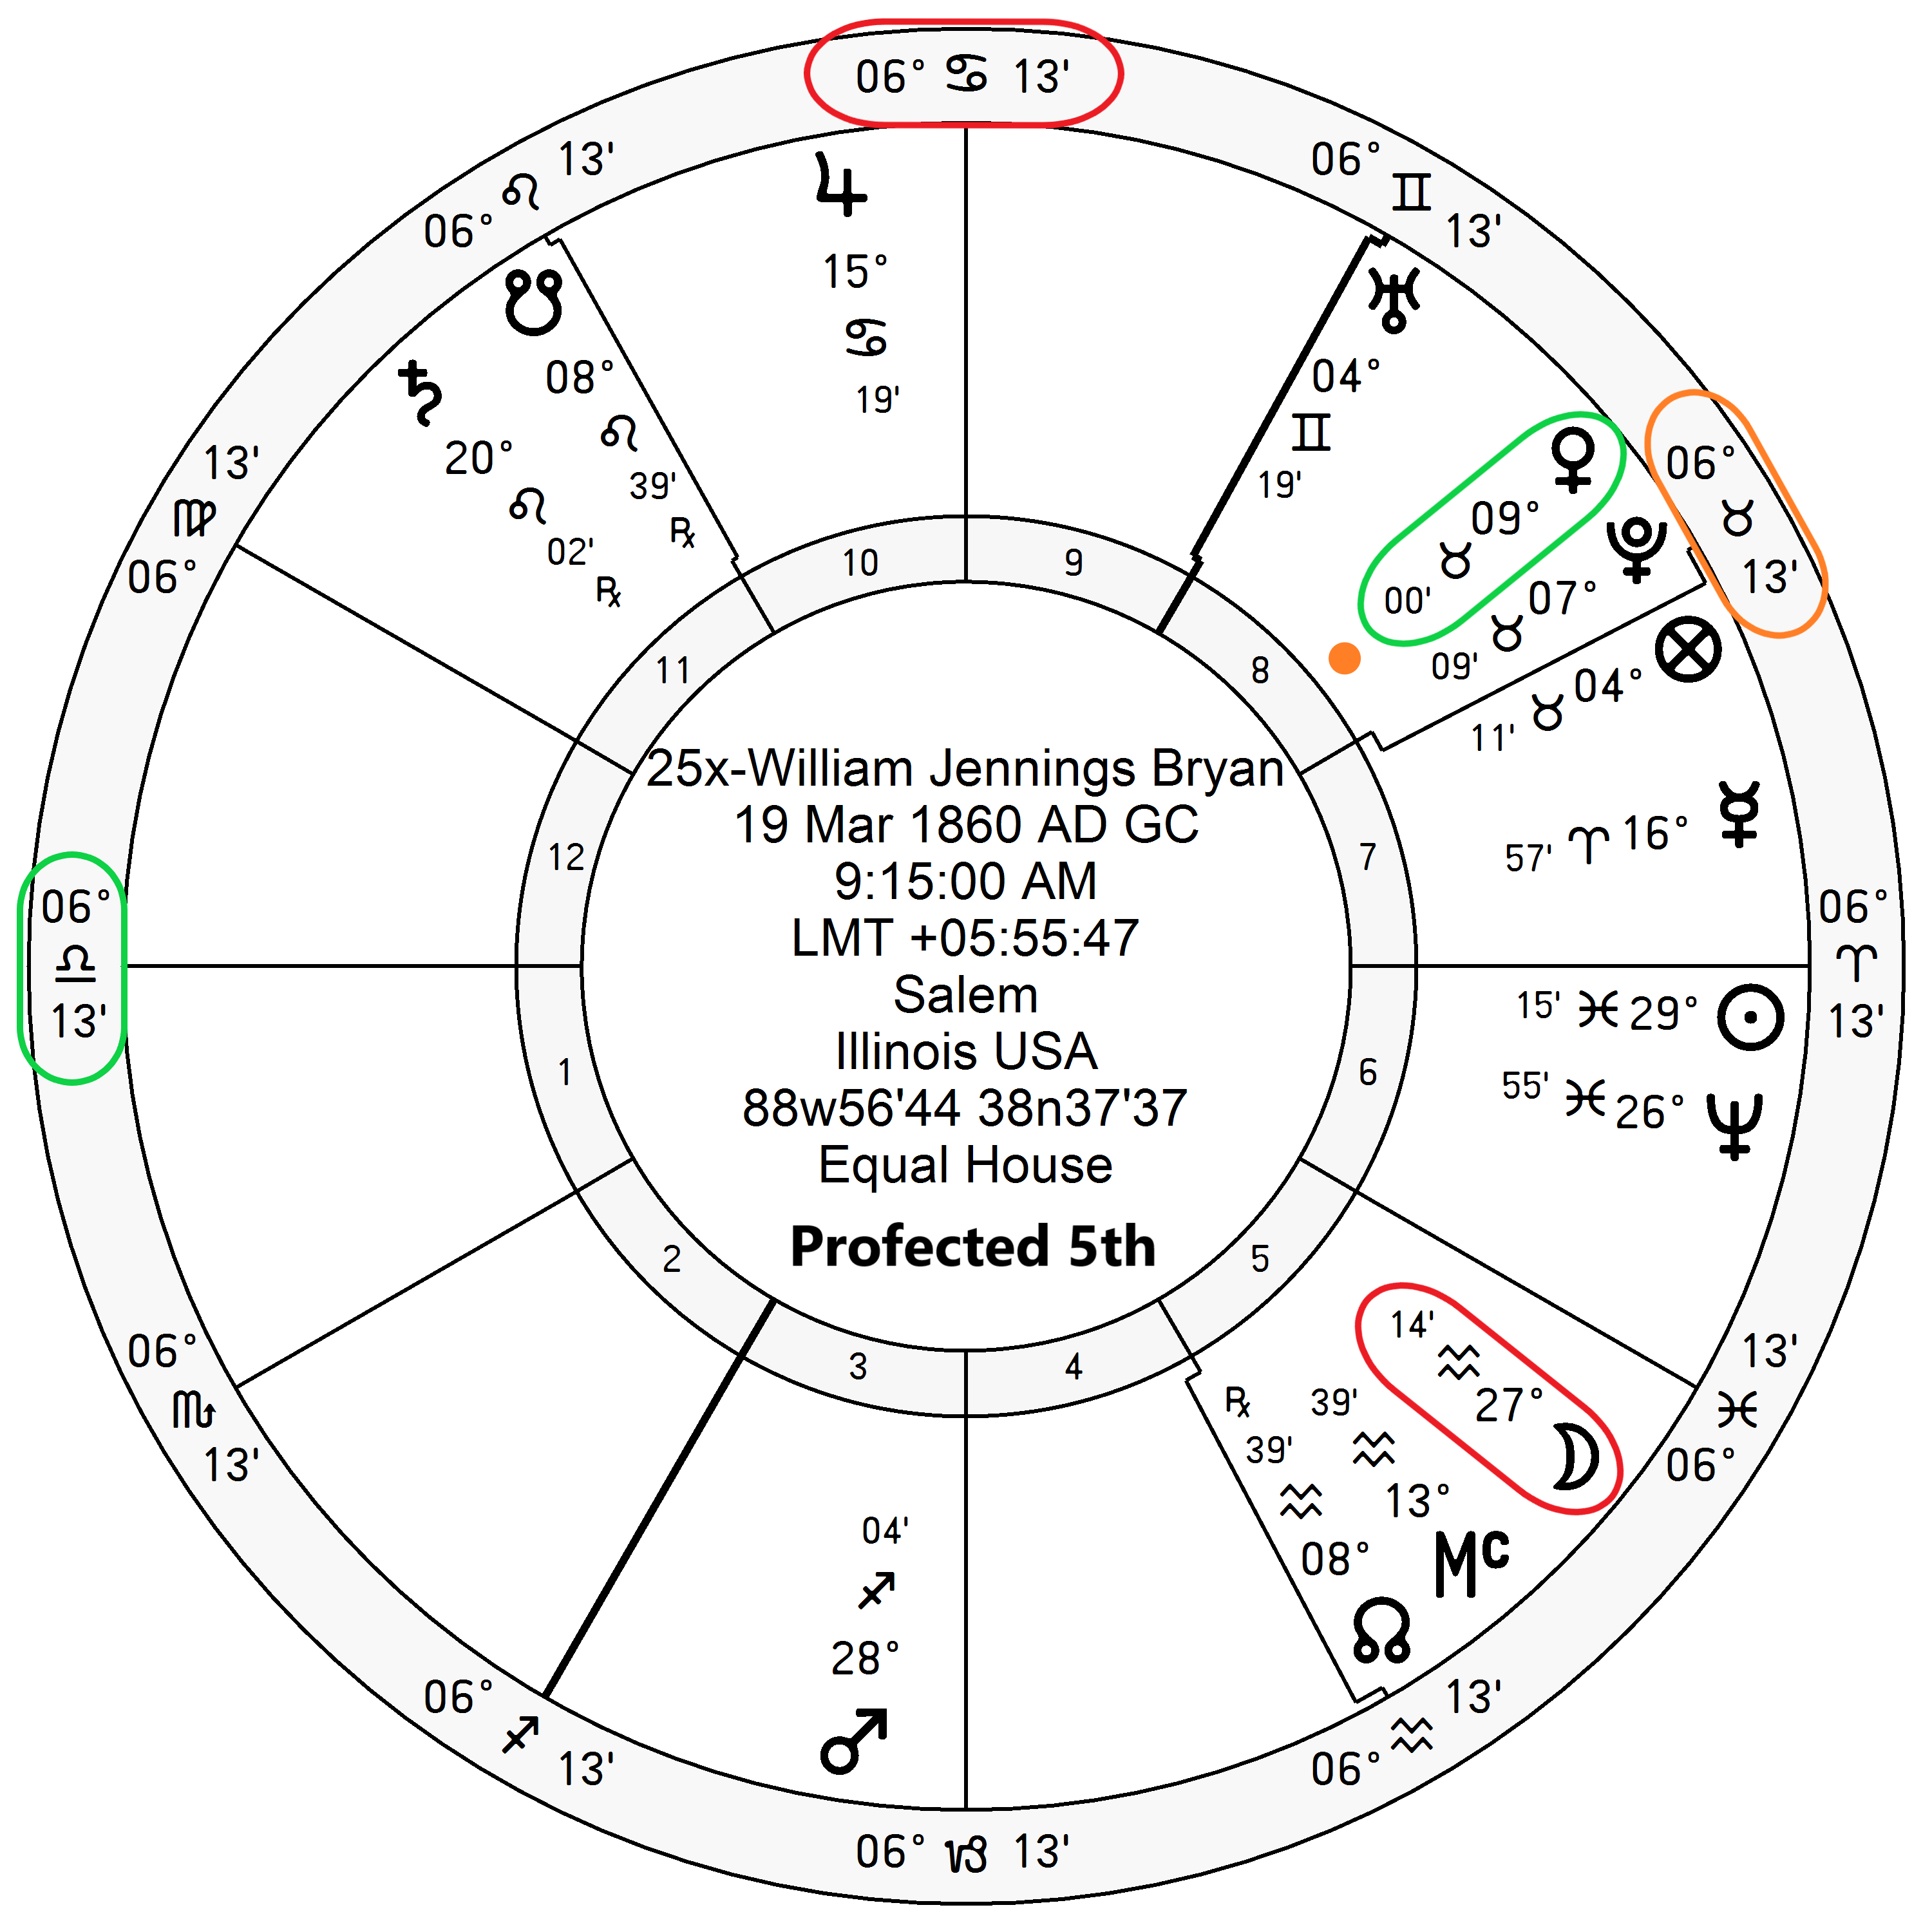
\includegraphics[width=0.9\textwidth]{charts/Bryan-Prof-5th.png}}
\textbf{\dgreen P1}=N6 
	$\Rightarrow$ \Venus\, $\Rightarrow$ \textbf{\dgreen P8/N12}\\
\textbf{\red P10}=N3
	$\Rightarrow$ \Moon\, $\Rightarrow$ P5/\textbf{\red N10}\\
PE=\textbf{\dgreen P8/N12}
	$\Rightarrow$ \Saturn\,\Retrograde $\Rightarrow$ \textbf{\dgreen P8/N12}

\end{columns}
\end{frame}
